\documentclass[tikz,border=5pt]{standalone}
\usepackage{amsmath}
\usepackage[american]{circuitikz}
\usetikzlibrary{arrows.meta,calc}
\definecolor{ink}{HTML}{16324F}
\definecolor{teal}{HTML}{168A88}
\definecolor{gold}{HTML}{D9892B}
\definecolor{redq}{HTML}{B84A4A}
\begin{document}
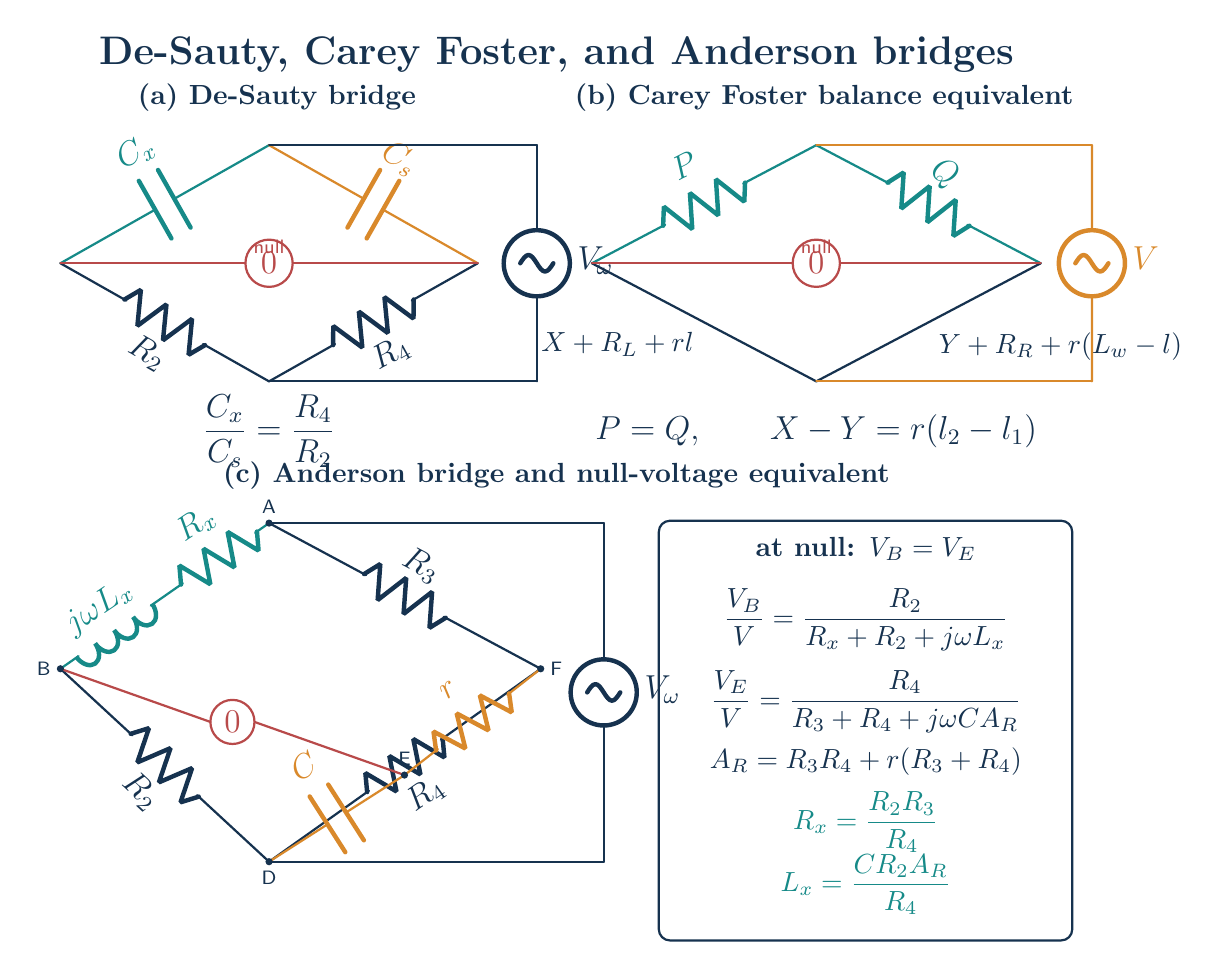
\begin{tikzpicture}[font=\large\sffamily,>=Latex,line cap=round,line join=round]
  \node[font=\bfseries\Large,ink] at (7.0,11.35)
    {De-Sauty, Carey Foster, and Anderson bridges};

  % De-Sauty
  \begin{scope}[shift={(.15,6.55)}]
    \node[font=\bfseries,ink] at (3.3,4.25) {(a) De-Sauty bridge};
    \coordinate (A) at (3.2,3.65);
    \coordinate (B) at (.55,2.15);
    \coordinate (C) at (3.2,.65);
    \coordinate (D) at (5.85,2.15);
    \draw[teal,thick] (A) to[C,l_=$C_x$] (B);
    \draw[ink,thick] (B) to[R,l_=$R_2$] (C);
    \draw[gold,thick] (A) to[C,l=$C_s$] (D);
    \draw[ink,thick] (D) to[R,l=$R_4$] (C);
    \coordinate (M) at ($(B)!.5!(D)$);
    \draw[redq,thick] (B)--($(M)+(-.30,0)$);
    \draw[redq,thick] ($(M)+(.30,0)$)--(D);
    \draw[redq,thick] (M) circle (.30) node {\(\,0\,\)};
    \node[redq,above] at (M) {\scriptsize null};
    \draw[ink,thick] (A)--(6.6,3.65) coordinate (As);
    \draw[ink,thick] (C)--(6.6,.65) coordinate (Cs);
    \draw[ink,thick] (As) to[sV,l=$V_\omega$] (Cs);
    \node[ink] at (3.2,.02)
      {$\displaystyle \frac{C_x}{C_s}=\frac{R_4}{R_2}$};
  \end{scope}

  % Carey Foster equivalent
  \begin{scope}[shift={(7.1,6.55)}]
    \node[font=\bfseries,ink] at (3.3,4.25) {(b) Carey Foster balance equivalent};
    \coordinate (A) at (3.2,3.65);
    \coordinate (B) at (.35,2.15);
    \coordinate (S) at (3.2,.65);
    \coordinate (D) at (6.05,2.15);
    \draw[teal,thick] (A) to[R,l_=$P$] (B);
    \draw[teal,thick] (A) to[R,l=$Q$] (D);
    \draw[ink,thick] (B)--node[below left,align=center,font=\normalsize]
      {$X+R_L+rl$} (S);
    \draw[ink,thick] (D)--node[below right,align=center,font=\normalsize]
      {$Y+R_R+r(L_w-l)$} (S);
    \coordinate (M) at ($(B)!.5!(D)$);
    \draw[redq,thick] (B)--($(M)+(-.30,0)$);
    \draw[redq,thick] ($(M)+(.30,0)$)--(D);
    \draw[redq,thick] (M) circle (.30) node {\(\,0\,\)};
    \node[redq,above] at (M) {\scriptsize null};
    \draw[gold,thick] (A)--(6.7,3.65) coordinate (As);
    \draw[gold,thick] (S)--(6.7,.65) coordinate (Ss);
    \draw[gold,thick] (As) to[sV,l=$V$] (Ss);
    \node[ink] at (3.2,.02)
      {$\displaystyle P=Q,\qquad X-Y=r(l_2-l_1)$};
  \end{scope}

  % Anderson bridge
  \begin{scope}[shift={(.35,.35)}]
    \node[font=\bfseries,ink] at (6.65,5.65)
      {(c) Anderson bridge and null-voltage equivalent};
    \coordinate (A) at (3.0,5.05);
    \coordinate (B) at (.35,3.20);
    \coordinate (D) at (3.0,.75);
    \coordinate (F) at (6.45,3.20);
    \coordinate (E) at (4.72,1.85);
    \draw[teal,thick] (A) to[R,l_=$R_x$] ($(A)!0.48!(B)$)
      to[L,l_=$j\omega L_x$] (B);
    \draw[ink,thick] (B) to[R,l_=$R_2$] (D);
    \draw[ink,thick] (A) to[R,l=$R_3$] (F);
    \draw[ink,thick] (F) to[R,l=$R_4$] (D);
    \draw[gold,thick] (F) to[R,l_=$r$] (E) to[C,l_=$C$] (D);
    \coordinate (M) at ($(B)!.5!(E)$);
    \draw[redq,thick] (B)--($(M)+(-.28,0)$);
    \draw[redq,thick] ($(M)+(.28,0)$)--(E);
    \draw[redq,thick] (M) circle (.28) node {\(\,0\,\)};
    \draw[ink,thick] (A)--(7.25,5.05) coordinate (As);
    \draw[ink,thick] (D)--(7.25,.75) coordinate (Ds);
    \draw[ink,thick] (As) to[sV,l=$V_\omega$] (Ds);
    \foreach \P/\lab/\pos in {A/A/above,B/B/left,D/D/below,F/F/right,E/E/above}
      \fill[ink] (\P) circle (1.3pt) node[\pos] {\scriptsize\lab};

    \draw[ink,thick,rounded corners] (7.95,-.25) rectangle (13.2,5.08);
    \node[font=\bfseries,ink] at (10.58,4.72) {at null: \(V_B=V_E\)};
    \node[ink,align=center,font=\normalsize] at (10.58,3.82)
      {$\displaystyle \frac{V_B}{V}=
        \frac{R_2}{R_x+R_2+j\omega L_x}$};
    \node[ink,align=center,font=\normalsize] at (10.58,2.78)
      {$\displaystyle \frac{V_E}{V}=
        \frac{R_4}{R_3+R_4+j\omega C A_R}$};
    \node[ink,font=\normalsize] at (10.58,2.02)
      {$A_R=R_3R_4+r(R_3+R_4)$};
    \node[teal,font=\normalsize] at (10.58,1.25)
      {$\displaystyle R_x=\frac{R_2R_3}{R_4}$};
    \node[teal,font=\normalsize] at (10.58,.46)
      {$\displaystyle L_x=\frac{CR_2A_R}{R_4}$};
  \end{scope}
\end{tikzpicture}
\end{document}
